\documentclass[french,a4paper,addpoints,11pt,answers]{exam}
\usepackage{hexercises-series}
\usepackage{mathtools, nccmath}
\usepackage{tabularx}
\title{La récursivité}
\seriesno{\texttt{0x25}}
\department{TIN}
\classroom{INFO2-TIN}

\begin{document}
\maketitle

\ifprintanswers
\else
\begin{multicols}{2}
\fi
\begin{questions}

\question
On considère la suite de Fibonacci, définie par la relation suivante:

\[
    \left\{\begin{matrix}
        f_0 & = & 0\\
        f_1 & = & 1\\
        f_n & = & f_{n-1}+f_{n-2}
        \end{matrix}\right.
\]

\begin{parts}
\part Écrire une fonction récursive qui calcule le terme de rang $n$ de cette suite.

\begin{solution}
Il est nécessaire de rajouter des parenthèses dans la définition de la macro.
\begin{lstlisting}
int fib(unsigned int n) {
  if (n == 0 || n == 1) return n;
  return fib(n - 1) + fib(n - 2);
}
\end{lstlisting}
\end{solution}

\part Représentez par un arbre les appels de fonction imbriqués lors de l'évaluation pour l'appel de \CD{fib(7)}.

\begin{solution}
    On peut établir le diagramme d'appel suivant:\par
\begin{center}
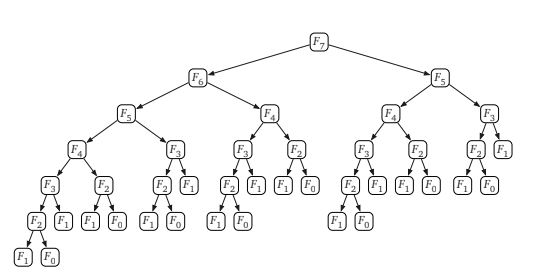
\includegraphics[width=10cm]{assets/fib.png}
\end{center}
\end{solution}

\part Quelle est la complexité en temps (\emph{big-O}) de cette fonction ?

\begin{solution}
Pour l'appel de \CD{fib(7)} on peut voir le nombre d'appels suivants.

\begin{tabular}{ll}
$n$ & Appels \\
0 & 1 \\
1 & 1 \\
2 & 3 \\
3 & 5 \\
4 & 9 \\
5 & 15 \\
6 & 25 \\
7 & 40 \\
\end{tabular}

La complexité en temps de cette fonction est exponentiel. Rappelons l'équation de la suite de fibonacci :

\[
f(n) = f(n - 1) + f (n - 2)
\]

Son équation caractéristique est :

\[
x^2 = x + 1\\
x^2 - x - 1 = 0
\]

Donc, la résolution par la relation quadratique donne les racines suivantes:

\[
    x_{1,2} = \left\{\begin{matrix}
        (1+\sqrt{5})/2 \\
        (1-\sqrt{5})/2 \\
        \end{matrix}\right.
\]

On sait que pour une solution linaire récursive est donné par :

\[
f(n) = \alpha_1^2 + \alpha_1^2
\]

où, $\alpha_1$ et $\alpha_2$ sont les racines de l'équation caractéristique. De cette assertion, on peut considérer que la complexité en temps est donnée par:
\[
O((1+\sqrt{5}/2)^n + ((1-\sqrt{5})/2)^2) = O(1.618^n) \rightarrow O(2^n)
\]

\end{solution}

\part Écrire une fonction itérative qui calcule le terme de rang $n$

\begin{solution}
Il est nécessaire de rajouter des parenthèses dans la définition de la macro.
\begin{lstlisting}
int fib_iterative(unsigned int n) {
  int result, first = 0, second = 1;
  for (i = 0; i < n; i++) {
    if (i <= 1)
      result = i;
    else {
      result = first + second;
      first = second;
      second = result;
    }
  }
  return result;
}
\end{lstlisting}
\end{solution}

\part Quelle est la complexité en temps de cette fonction itérative ?

\begin{solution}
On ne voit ici qu'une seule boucle parcourant les valeurs de 0 à $n$. Dès lors la complexité en temps est de :

\[
O(n)
\]
\end{solution}

\part Écrire une fonction de mémoization en programmation dynamique qui  encapsule votre fonction récursive afin de réduire la complexité.

\begin{solution}
La mémoization est une technique permettant de mémoriser les résultats des appels d'une fonction récursive. Ceci permet de réduire la complexité de traitement en utilisant davantage de mémoire.
\begin{lstlisting}
#define FIB_CACHE_SIZE 100
int fib_cache[FIB_CACHE_SIZE] = {};
int fib_mem(unsigned int n) {
    assert(n < FIB_CACHE_SIZE);
    if (fib_cache[n] > 0)
        return fib_cache[n];
    int result = fib(n);
    fib_cache[n] = result;
    return result;
}
\end{lstlisting}
\end{solution}
\part Quelle est la complexité de cette nouvelle fonction ?

\begin{solution}
La complexité devient $O(n)$ temps avec une complexité de $O(n)$ en espace mémoire.
\end{solution}

\end{parts}

\question
Pour réaliser certaines fonctions de calcul dans une application de simulation numérique, on doit disposer d'une fonction calculant le polynôme suivant :
\[
p(x) = \frac{0\cdot x^0}{0!} + \frac{1\cdot x^1}{1!} + \frac{2\cdot x^2}{2!} + \frac{3\cdot x^3}{3!} + \frac{4\cdot x^4}{4!} + \frac{5\cdot x^5}{5!}
\]

Le calcul de ce polynôme a été programmé de la façon suivante dans cette application :
\lstinputlisting{polynome.c}

Cette fonction est appelée des millions de fois pendant le calcul de la simulation numérique, et les temps de calcul obtenus sont beaucoup trop élevés.

\begin{parts}
    \part Expliquez pourquoi la programmation de cette fonction n'est pas optimale au niveau des performances.

\begin{solution}
    La factorielle de 1 à 5 est recalculée des millions de fois, alors que c'est une valeur constante.
    Le calcul du polynôme est fait avec la méthode inefficace des puissances. Ainsi, on ne réutilise pas la valeur de $x^2$ pour calculer $x^3$.
\end{solution}

    \part Proposez des optimisations du code permettant de diminuer significativement les temps de calcul de cette fonction.
\begin{solution}
Après simplification, on voit que cette fonction peut être calculée de façon beaucoup plus simple et efficace sous la forme suivante :

\begin{lstlisting}
double calcul_polynome2(double x)
{
  return x * (1.0 + x * (1.0 + x * (0.5 + x * ((1/6.0) + x *
     (1/24.)))));
}
\end{lstlisting}
\end{solution}
\end{parts}

\end{questions}

\ifprintanswers
\else
\end{multicols}
\fi
\end{document}
